\documentclass[12pt]{article}
\usepackage{amsmath,amsthm,amssymb,amsfonts,bm}
\usepackage{graphicx,color}
\usepackage{epstopdf}
\usepackage[margin=1in]{geometry} 
\graphicspath{{~/Documents/school/fall16/stat586/final/html}}
\setcounter{secnumdepth}{0}

\sloppy
\definecolor{lightgray}{gray}{0.5}
 
\newcommand{\N}{\mathbb{N}}
\newcommand{\Z}{\mathbb{Z}}
\newcommand{\normD}[3]{\frac{1}{\sqrt{2\pi #1^2}}exp\left(\frac{-( #2 - #3)^2}{2 #1^2}\right)} 
\newcommand{\cProb}[2]{P(#1|#2)}
\newcommand{\infSum}{\lim_{n\to\infty} \sum_{n=i}^\infty}

\begin{document}
\title{Final}
\author{Taylor Bodin}
\maketitle

\section{Question 1}
\subsection{Inverse Transformation}
\begin{align*}
u &= x + y \\
v &= x - y \\
x &= \frac{u+v}{2} \\
y &= \frac{u-v}{2}
\end{align*}

\subsection{Jacobian}
\begin{align*}
  J &= det\begin{bmatrix}
    \frac{\delta x}{\delta u} & \frac{\delta x}{\delta v} \\
    \frac{\delta y}{\delta u} & \frac{\delta y}{\delta v}
  \end{bmatrix} \\
  &= det\begin{bmatrix}
    \frac{1}{2} & \frac{1}{2} \\
    \frac{1}{2} & -\frac{1}{2} \\
  \end{bmatrix} \\
  &= -\frac{1}{2}
\end{align*}

\subsection{Transform}
\begin{align*}
  f_{X,Y}(x,y) = f_X(x)f_Y(y) = f_{X,Y}(x,y) &= \frac{1}{2\pi\sigma^2}
  exp\left( -\frac{(x-\mu)^2}{2\sigma^2} \right)
  exp\left( -\frac{(y-\tau)^2}{2\sigma^2} \right) \\
  f_{U,V}(u,v) = f_{X,Y}(h_1(u,v),h_2(u,v))|J| &= \frac{1}{2\pi2\sigma^2}
  exp\left( -\frac{(\frac{u+v}{2}-\mu)^2}{2\sigma^2} \right)
  exp\left( -\frac{(\frac{u-v}{2}-\tau)^2}{2\sigma^2} \right) \\
  \left( \frac{u+v}{2}-\mu \right)^2 + \left( \frac{u-v}{2}-\tau \right)^2 
    &= \frac{1}{2}\left((u^2 -2u(\mu+\tau) +\mu^2 +\tau^2) + (v^2 -2v(\mu-\tau) +\mu^2 +\tau^2)\right) \\
    &= \frac{1}{2}\left( u-(\mu+\tau) \right)^2 + \frac{1}{2}\left( v - (\mu-\tau) \right)^2 \\
  f_{U,V}(u,v) &= \frac{1}{2\pi2\sigma^2}
  exp\left( -\frac{(u-(\mu+\tau))^2}{2(2\sigma^2)} \right)
  exp\left( -\frac{(v-(\mu-\tau))^2}{2(2\sigma^2)} \right) \\
  f_U(u) &= \frac{1}{\sqrt{2\pi2\sigma^2}} exp\left( -\frac{(u-(\mu+\tau))^2}{2(2\sigma^2)} \right) \\
  U &\sim N((\mu+\tau),2\sigma^2) \\
  f_V(v) &= \frac{1}{\sqrt{2\pi2\sigma^2}} exp\left( -\frac{(v-(\mu-\tau))^2}{2(2\sigma^2)} \right) \\
  V &\sim N((\mu-\tau),2\sigma^2)
\end{align*}
Because U and V are seperable they are independent.

\section{Problem 2}
\subsection{Finding the parameters for \textbf{Y}}
Since the RVs in \textbf{Y} are zero mean, $Cov(Y_i,Y_j) = E[Y_iY_j] + \mu_i \mu_j = E[Y_i Y_j]$. Further when $i=j$, 
$E[Y_i^2] = \sigma_i^2 + \mu_i^2 = \sigma_i^2$. So the covariance matrix for this distribution contains the variances for
the RVs on the left diagonal and the Miller correlation between the RVs everywhere else. Using the values from the
covariance matrix it's possible to specify parameters for \textbf{X}. 

\subsection{a.}
\subsubsection{Find $X_1$}
Since $X_1$ is a sum of Gaussian RVs, it is also a Gaussian RV.
\begin{align*}
  E[X_1] &= E[Y_1 - Y_2] = E[Y_1] - E[Y_2] = 0 - 0 = 0 \\
  E[X_1^2] &= \sigma_{X_1}^2 + \mu_{X_1}^2 = \sigma_{X_1}^2 \\
  &= E[(Y_1-Y_2)^2] = E[Y_1^2] -2E[Y_1Y_2] + E[Y_2^2] = 1 - 2\rho +1 = 2-2\rho \\
  X_1 &\sim N(0,2-2\rho)
\end{align*}
\subsubsection{Find $X_2$}
Since $X_2$ is also a sum of Gaussian RVs, it is also a Gaussian RV.
\begin{align*}
  E[X_2] &= E[Y_2 - Y_3] = E[Y_2] - E[Y_3] = 0 - 0 = 0 \\
  E[X_1^2] &= \sigma_{X_2}^2 + \mu_{X_2}^2 = \sigma_{X_2}^2 \\
  &= E[(Y_2-Y_3)^2] = E[Y_2^2] -2E[Y_2Y_3] + E[Y_3^2] = 1 - 2\rho +1 = 2-2\rho \\
  X_2 &\sim N(0,2-2\rho)
\end{align*}
\subsubsection{Find $\Sigma_{\bm{X}}$}
\begin{align*}
  \Sigma_{\bm{X}} &= 
  \begin{bmatrix}
    2-2\rho & E[X_1X_2] \\
    E[X_2X_1] & 2-2\rho
  \end{bmatrix} \\
  E[X_1X_2] = E[X_2X_1] &= E[(Y_1-Y_2)(Y_2-Y_3] \\
  &= E[Y_1Y_2] - E[Y_2^2] - E[Y_1Y_3] + E[Y_2Y_3] \\
  &= \rho - 1 - 0 + \rho = 2\rho - 1 \\
  \Sigma_{\bm{X}} &= 
  \begin{bmatrix}
    2-2\rho & 2\rho - 1 \\
    2\rho - 1 & 2-2\rho
  \end{bmatrix} \\
\end{align*}
Thus, $\bm{X} \sim N_2(0,\Sigma_{\bm{X}})$
\subsection{b.}
If $\rho = \frac{1}{2}$ the covariance matrix for \textbf{X} goes to:
\[
  \begin{bmatrix}
    1 & 0 \\
    0 & 1
  \end{bmatrix}
\]
Which shows the covariance between $X_1$ and $X_2$ to be 0 and therefore the two RV are independent. 

\subsection{c.}
For a covariance matrix to be valid, it has to be positive definite. This means it must be symmetric and have positive eigenvalues.
The variances for the individual RVs are also strictly greater than 0.
\subsubsection{$\Sigma_{\bm{Y}}$}
The eigenvalues for $\Sigma_{\bm{Y}}$ are: $1, \frac{1}{4}\rho + 1, 1 - \frac{1}{4}\rho$. Thus for $\rho < 4$ the covariance matrix
will be valid. Since the variances in \textbf{Y} are all 1, $\rho$ is bounded by $[-1,1]$ and thus can't take on a value of 4. Therefore
the covariance matrix is valid everywhere.

\subsubsection{$\Sigma_{\bm{X}}$}
The eigenvalues for $\Sigma_{\bm{X}}$ are: $1, 3 - 4\rho$. Thus for $\rho < 3/4$ the covariance matrix will be valid. 

\section{Problem 3}
\subsection{Inverse Transformation}
\begin{align*}
  u &= \frac{x}{x + y} \\
  v &= \frac{x + y}{x+y+z} \\
  w &= \frac{x + y}{x+y+z} \\
  x &= uvw \\
  y &= vw - uvw \\
  z &= w - vw \\
\end{align*}

\subsection{Jacobian}
\begin{align*}
  J &= det\begin{bmatrix}
    \frac{\delta x}{\delta u} & \frac{\delta x}{\delta v} & \frac{\delta x}{\delta w} \\
    \frac{\delta y}{\delta u} & \frac{\delta y}{\delta v} & \frac{\delta y}{\delta w}
    \frac{\delta z}{\delta u} & \frac{\delta z}{\delta v} & \frac{\delta z}{\delta w}
  \end{bmatrix} \\
  &= det\begin{bmatrix}
    vw & uw & uv \\
    -vw & w-uw & v-uv \\
    0 & -w & 1-v \\
  \end{bmatrix} \\
  &= vw^2
\end{align*}

\subsection{Transform}
\begin{align*}
  f_{X,Y,Z}(x,y,z) &= f_X(x)f_Y(y)f_Z(z) \\
  f_{U,V,W}(u,v,w) &= f_{X,Y,Z}(h_1(u,v,w),h_2(u,v,w)h_3(u,v,w))|J| \\
  &= vw^2exp(-w) \\
  f_U(u) &= 1 \\
  U &\sim Unif(0,1) \\
  f_V(v) &= 2v \\
  V &\sim \beta(2,1) \\
  f_W(w) &= \frac{w^2}{2}exp(-w) \\
  w &\sim \Gamma(3,1)
\end{align*}
Because U, V, W are seperable they are independent.

\section{Problem 4}
\subsection{Results}
\begin{table}[h]
\centering
\caption{Results}
\label{p4_data}
\begin{tabular}{|l|l|l|l|l|l|l|l|}
  \hline 
n  & mean & variance & skewness & 0.025 quantile & 0.975 quantile & lower CI & upper CI \\
\hline
10 &      &          &          &                &                &          &          \\
\hline
20 &      &          &          &                &                &          &          \\
\hline
40 &      &          &          &                &                &          &          \\
\hline
80 &      &          &          &                &                &          &         \\
\hline
\end{tabular}
\end{table}
\subsection{Discussion}
\subsection*{Contents}

\begin{itemize}
\setlength{\itemsep}{-1ex}
   \item Final Problem 4
   \item A. Generate the population of Gamma RVs
   \item B Part 1: Create Sample Distributions of Size n
\end{itemize}


\subsection*{Final Problem 4}

\begin{par}
Taylor Bodin 9 Dec 2016
\end{par} \vspace{1em}
\begin{verbatim}
% Setup Variables
clear; close all; clc;
set(0,'DefaultFigureWindowStyle','docked')

N = 500000; %Number of RV in the population
num_bins = 50; %Standard number of bins for histograms
n = [10 20 40 80 100 200 500];
ci = .975;
\end{verbatim}


\subsection*{A. Generate the population of Gamma RVs}

\begin{verbatim}
pop = random('Gamma',1,1,[1,N]);

% Descripitive Stats
mu = mean(pop); % Given
var = std(pop)^2;
skew = skewness(pop);
pop_quant_upper = quantile(pop,ci);
pop_quant_lower = quantile(pop,1-ci);

pop_stat_str = {['\mu = ', num2str(mu)];
    ['\sigma^2 = ' num2str(var)];
    ['Skew = ' num2str(skew)];
    ['Upper Quantile: ' num2str(pop_quant_upper)];
    ['Lower Quantile: ' num2str(pop_quant_lower)]};


% Population Figure
f1 = figure(1);

% Histogram
pop_hist = histogram(pop);
pop_hist.Normalization = 'PDF';
pop_hist.NumBins = num_bins;

% Quantiles
line([pop_quant_lower pop_quant_lower], get(gca, 'ylim'),...
    'Color', 'Red', 'LineWidth', 2, 'LineStyle', '--');
line([pop_quant_upper pop_quant_upper], get(gca, 'ylim'),...
    'Color', 'Green', 'LineWidth', 2, 'LineStyle', '--');

% Annotation
dim = [.4 .3 .3 .3];
annotation('textbox',dim,'String',pop_stat_str,'FitBoxToText','on');

% Figure Properties
title('Simulated PDF of the Gamma(1,1) RV')
xlabel('RV value');
f1.CurrentAxes.XAxis.Limits = [0 4];
ylabel('Probability Density');
legend('Gamma(1,1) PDF', 'Lower Quantile (.025)', 'Upper Quantile (.975)');
\end{verbatim}

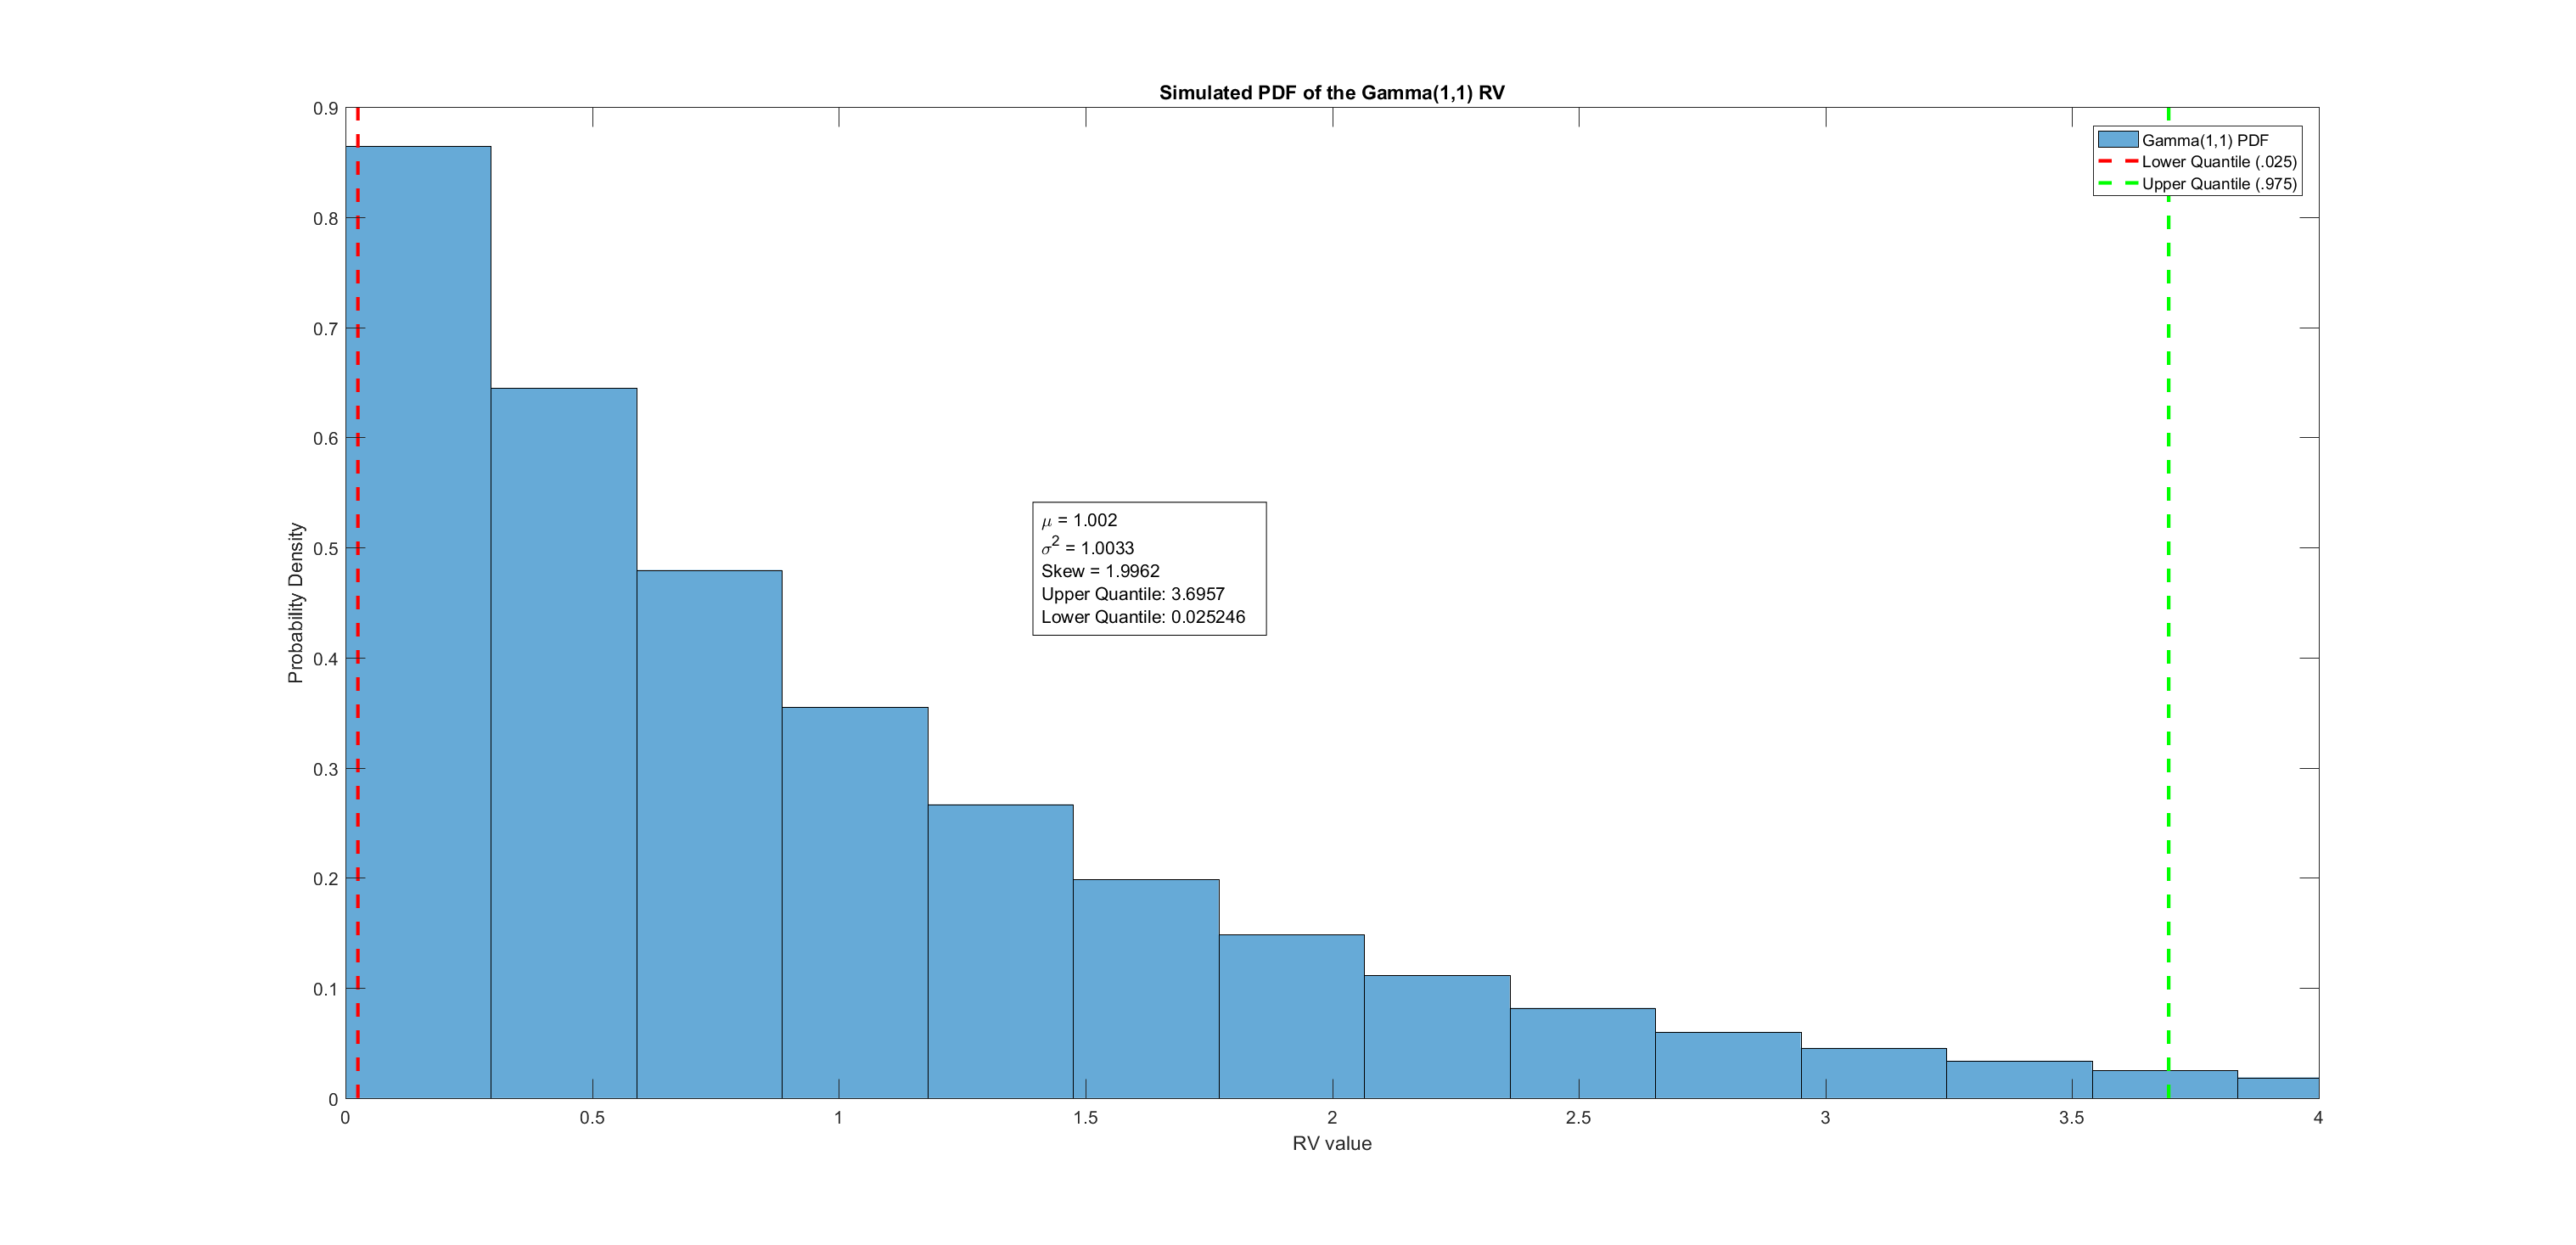
\includegraphics [width=\textwidth]{prob4_01.eps}


\subsection*{B Part 1: Create Sample Distributions of Size n}

\begin{verbatim}
for k=1:length(n)

sample = reshape(pop,n(k),[]);
sample = sample(:,1:1000); % Per the instructions only want 1000

% Descriptive Stats
s_mu = mean(sample);
mu_var = mean(std(s_mu).^2);
mu_skew = mean(skewness(s_mu));
s_quant_upper = mean(quantile(s_mu,ci));
s_quant_lower = mean(quantile(s_mu,1-ci));
ci_upper = mean(s_mu + sqrt(var/n(k))*qfuncinv((1-ci)/2));
ci_lower = mean(s_mu - sqrt(var/n(k))*qfuncinv((1-ci)/2));

% Summary of Descriptive Stats
s_stat_str = {['\mu = ', num2str(mean(s_mu))];
    ['\sigma^2 = ' num2str(mu_var)];
    ['Skew = ' num2str(mu_skew)];
    ['Upper Quantile: ' num2str(s_quant_upper)];
    ['Lower Quantile: ' num2str(s_quant_lower)]};

% Central Limit Theorem Approximation
cl_pd = makedist('Normal', 'mu', mu, 'sigma', var/sqrt(n(k)));
range = 0:.01:2.5;
cl_pdf = pdf(cl_pd,range);

% Create the figure
f2 = figure(k+1);
hold on
% -- Mean Histogram
s_hist = histogram(s_mu);
s_hist.Normalization = 'PDF';
s_hist.NumBins = num_bins;

xlims = f2.CurrentAxes.XAxis.Limits; %Need these xlims scaled for the hist

% -- Quantiles
q1 = line([s_quant_lower s_quant_lower], get(gca, 'ylim'),...
    'Color', 'Green', 'LineWidth', 2, 'LineStyle', '--');
q2 = line([s_quant_upper s_quant_upper], get(gca, 'ylim'),...
    'Color', 'Green', 'LineWidth', 2, 'LineStyle', '--');

% -- Central Limit Approximation
p1 = plot(range,cl_pdf, 'LineWidth', 2, 'LineStyle', '-.');

% -- Confidence Intervals
ci_1 = line([ci_lower ci_lower], get(gca, 'ylim'),...
    'Color', 'Red', 'LineWidth', 2, 'LineStyle', '--');
ci_2 = line([ci_upper ci_upper], get(gca, 'ylim'),...
    'Color', 'Red', 'LineWidth', 2, 'LineStyle', '--');

% -- Descripitve Annotation
dim = [.815 .52 .3 .3];
a1 = annotation('textbox',dim,'String',s_stat_str,'FitBoxToText','on');

% -- Figure Properties
f2.CurrentAxes.XAxis.Limits = xlims;
title(['PDF of Sample Means of Sample Size ' num2str(n(k))])
xlabel('Value of \mu');
ylabel('Probability Density');
legend([s_hist q1 p1 ci_1], ...
    ['PDF of \mu_{N=' num2str(n(k)) '}'], '97.5% Quantiles'...
    ,'Central Limit Approximation', '97.5% Confidence Intervals');
hold off
end
\end{verbatim}

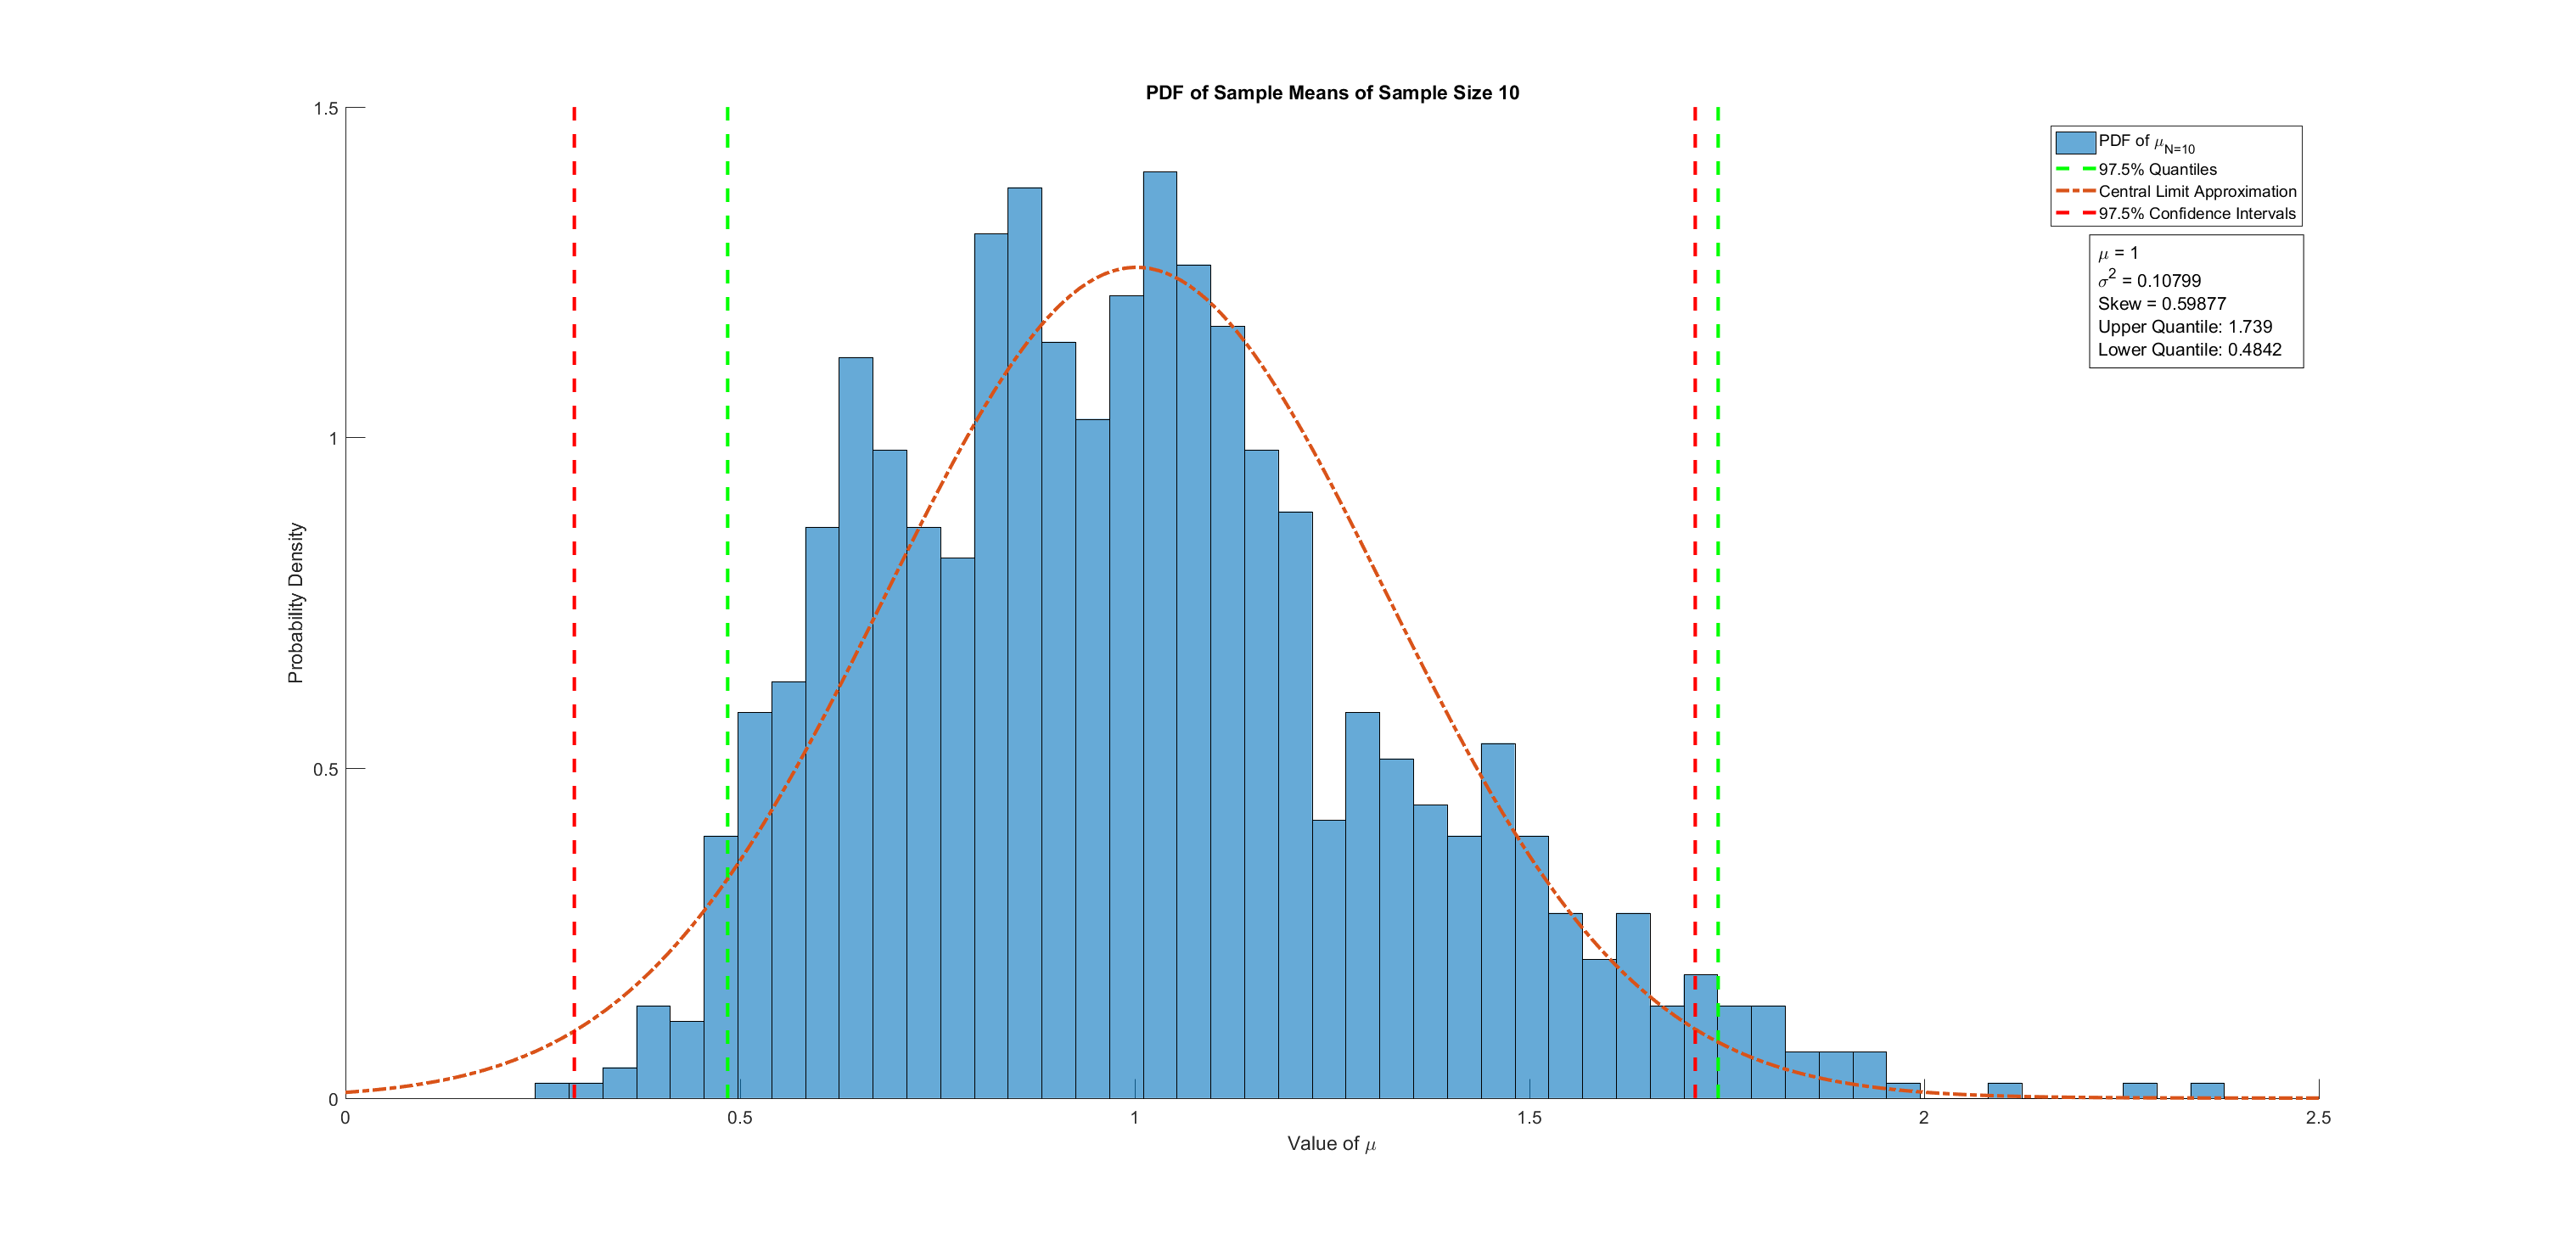
\includegraphics [width=\textwidth]{prob4_02.eps}

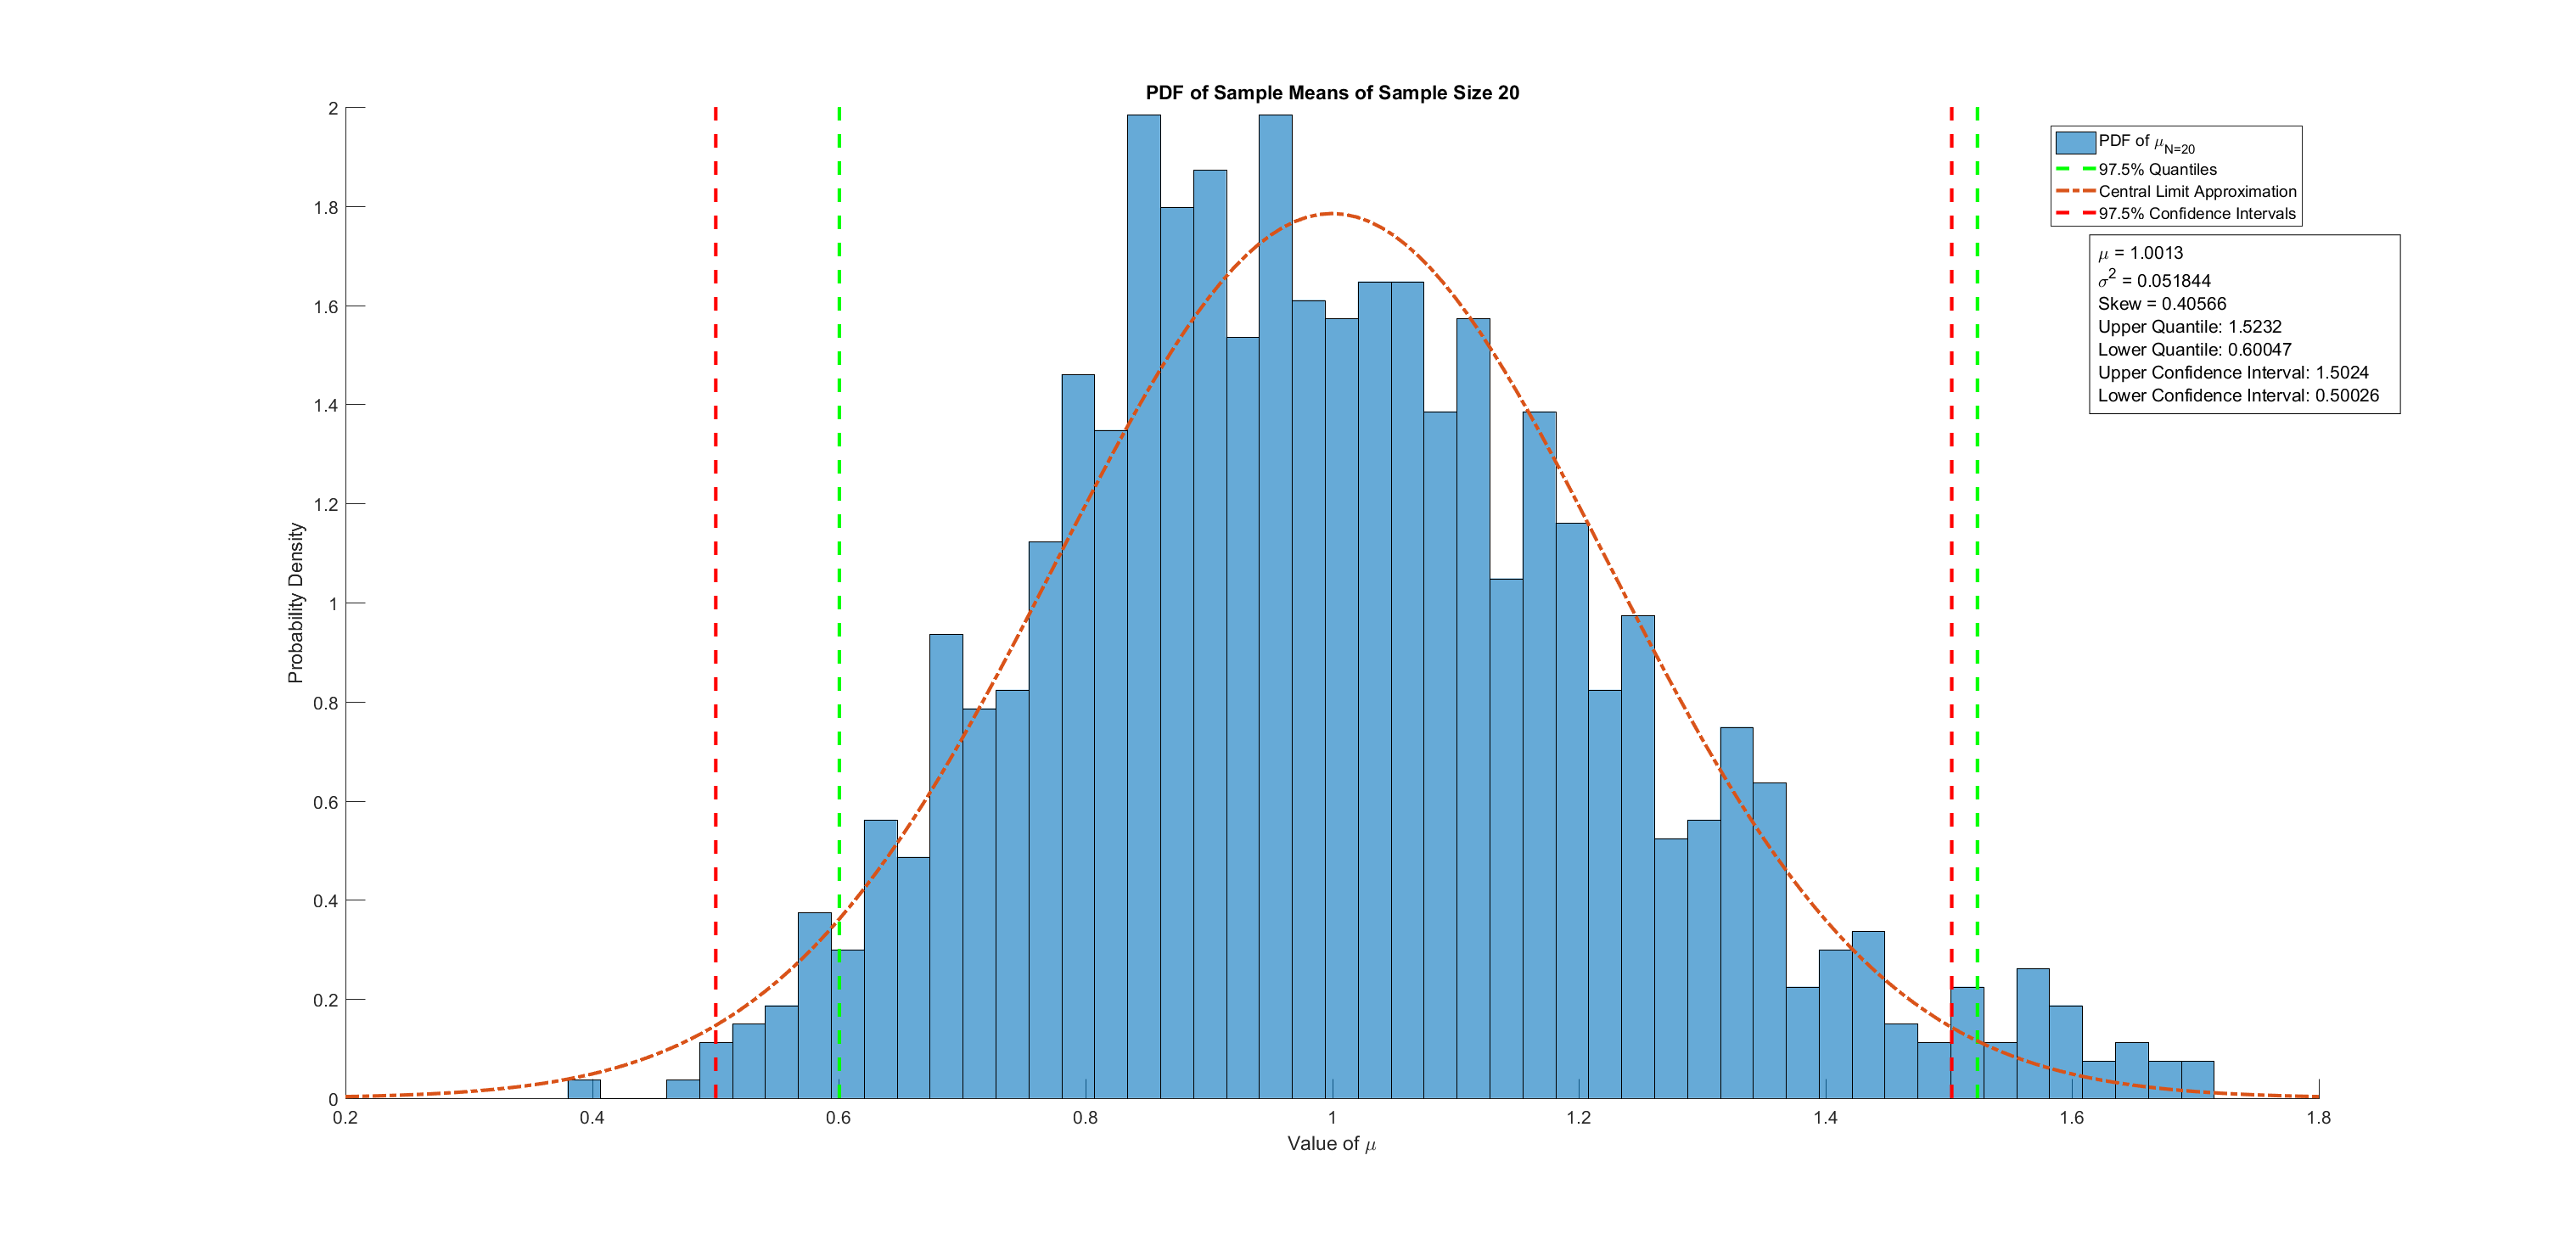
\includegraphics [width=\textwidth]{prob4_03.eps}

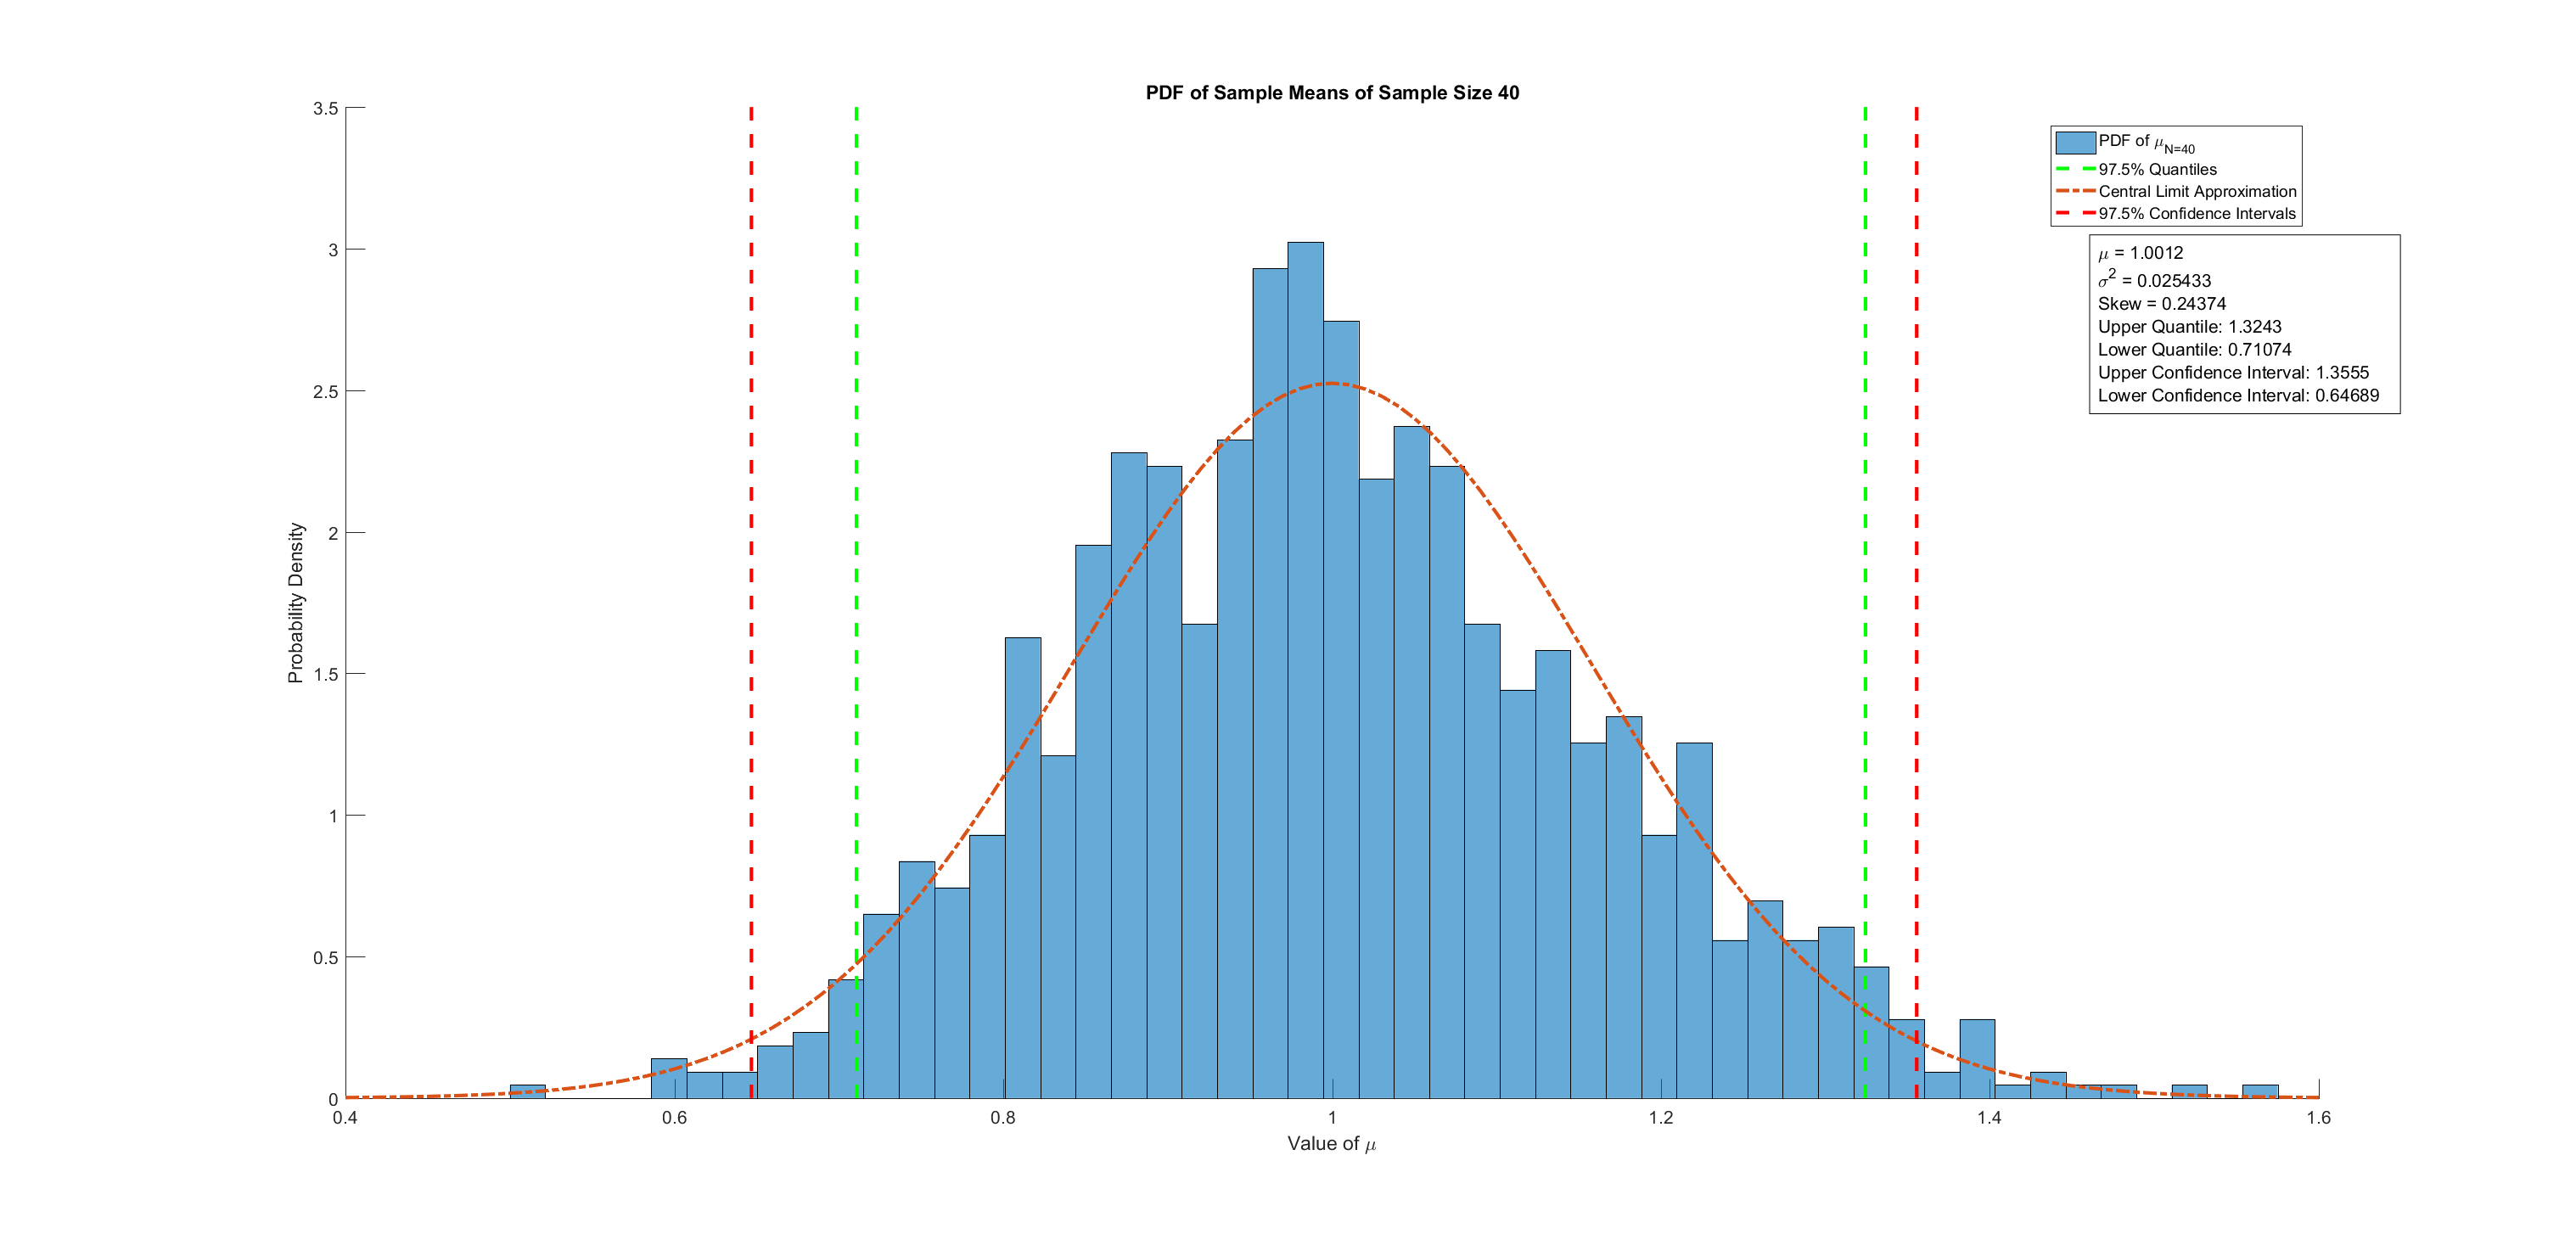
\includegraphics [width=\textwidth]{prob4_04.eps}

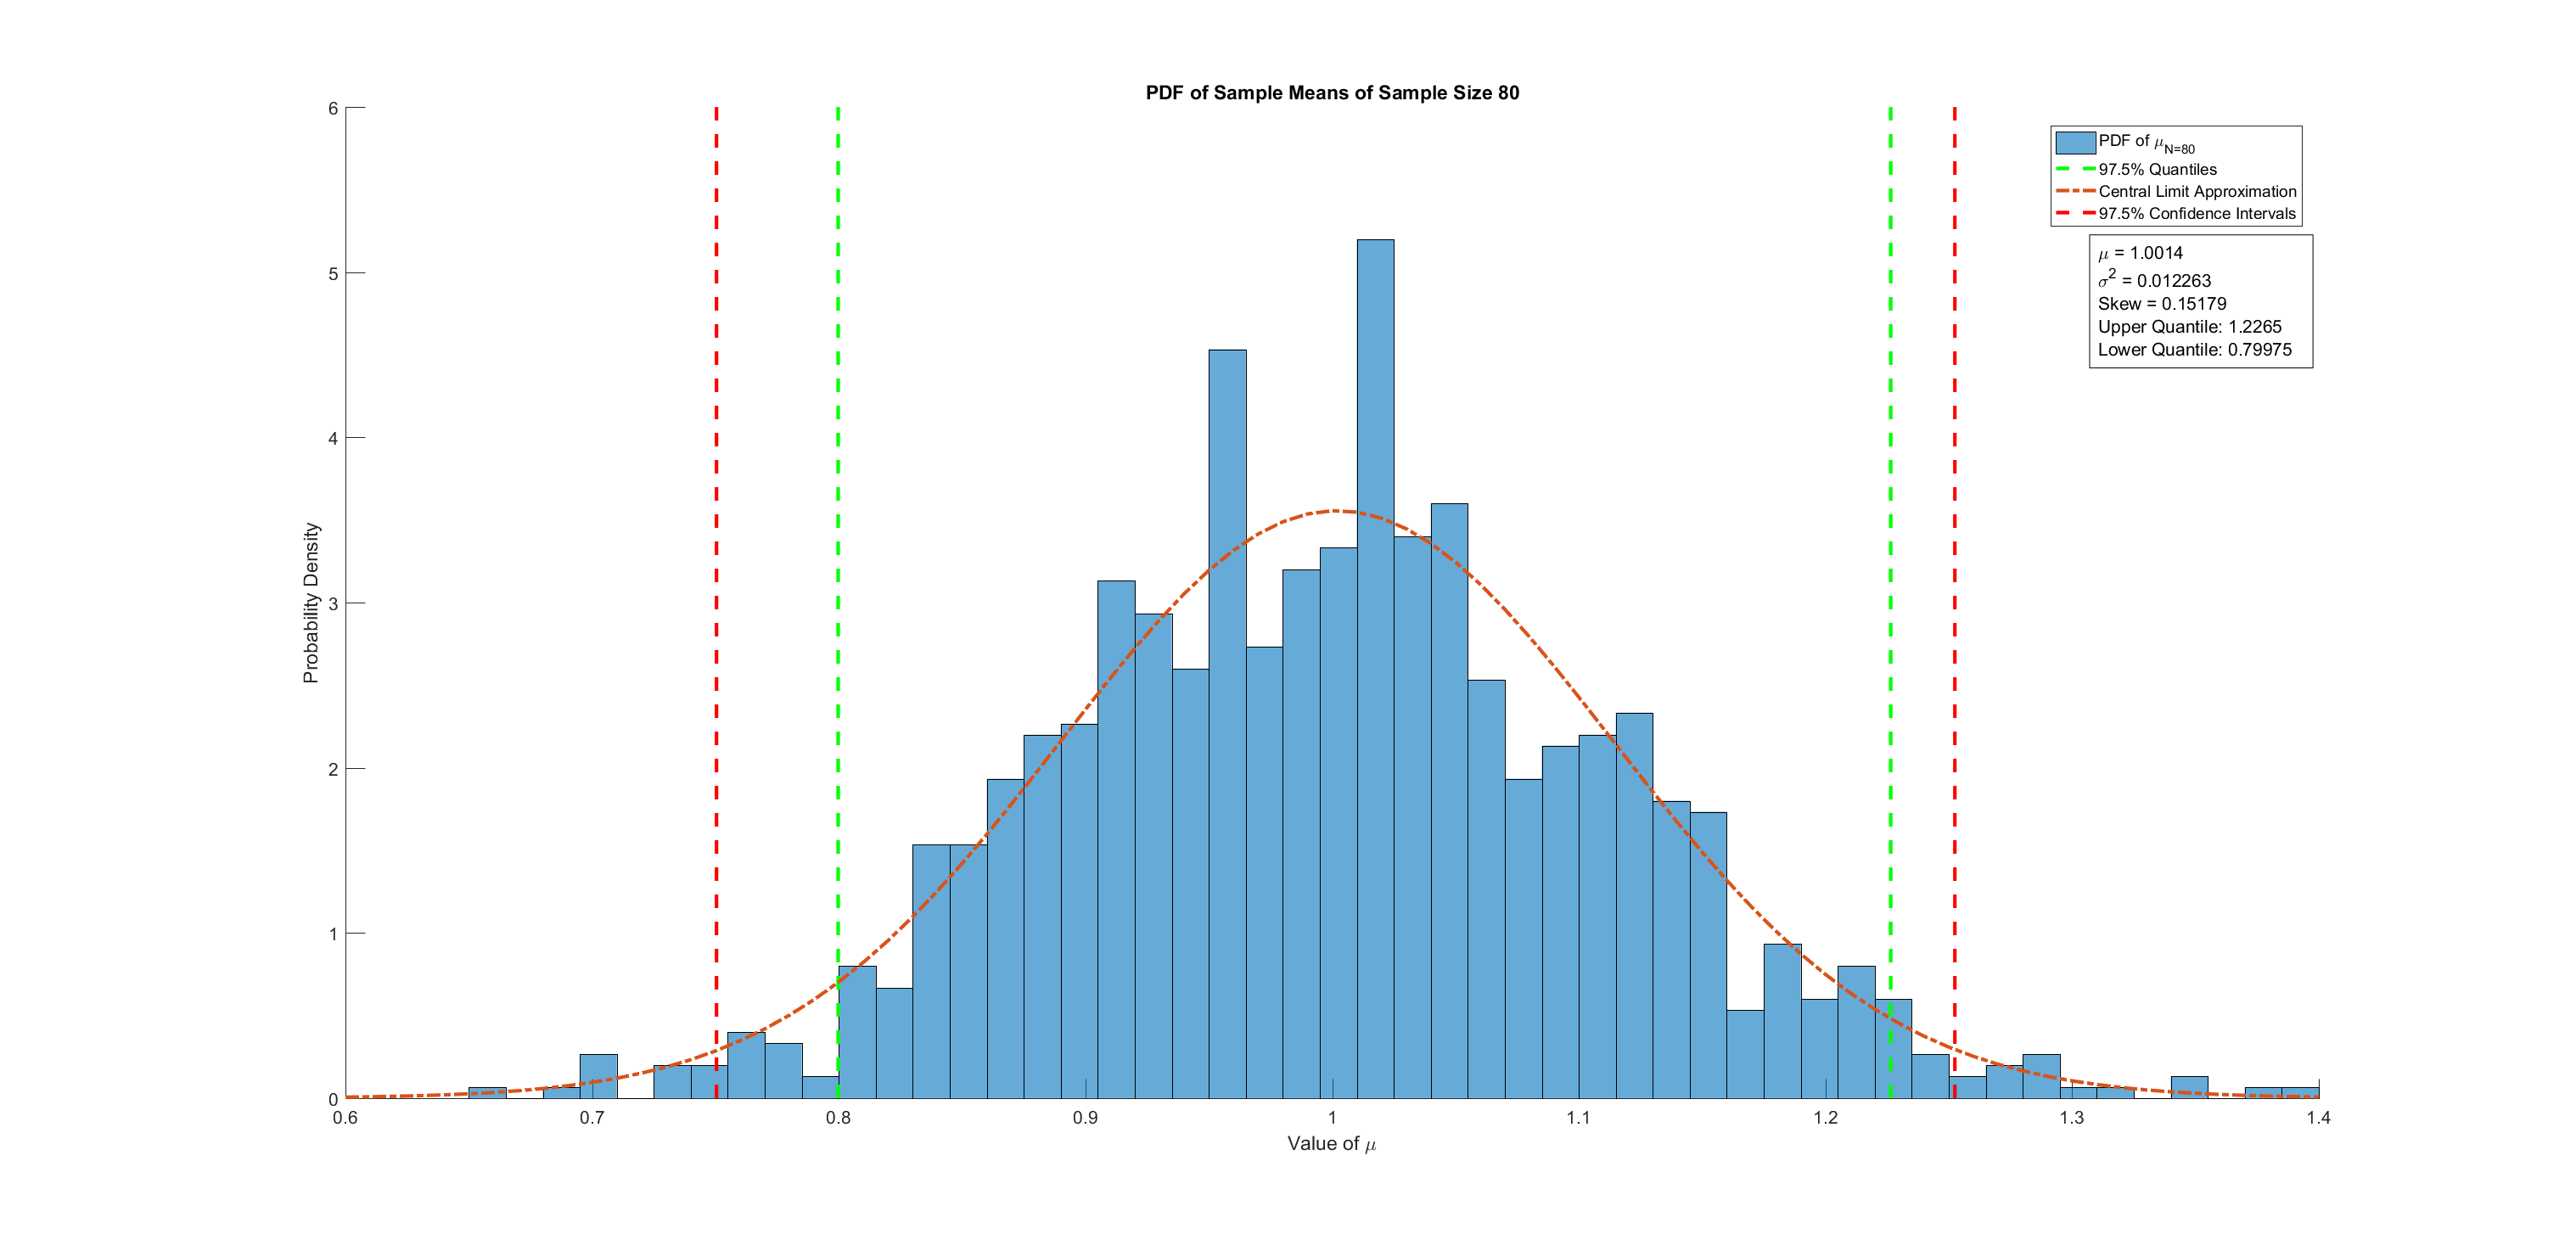
\includegraphics [width=\textwidth]{prob4_05.eps}

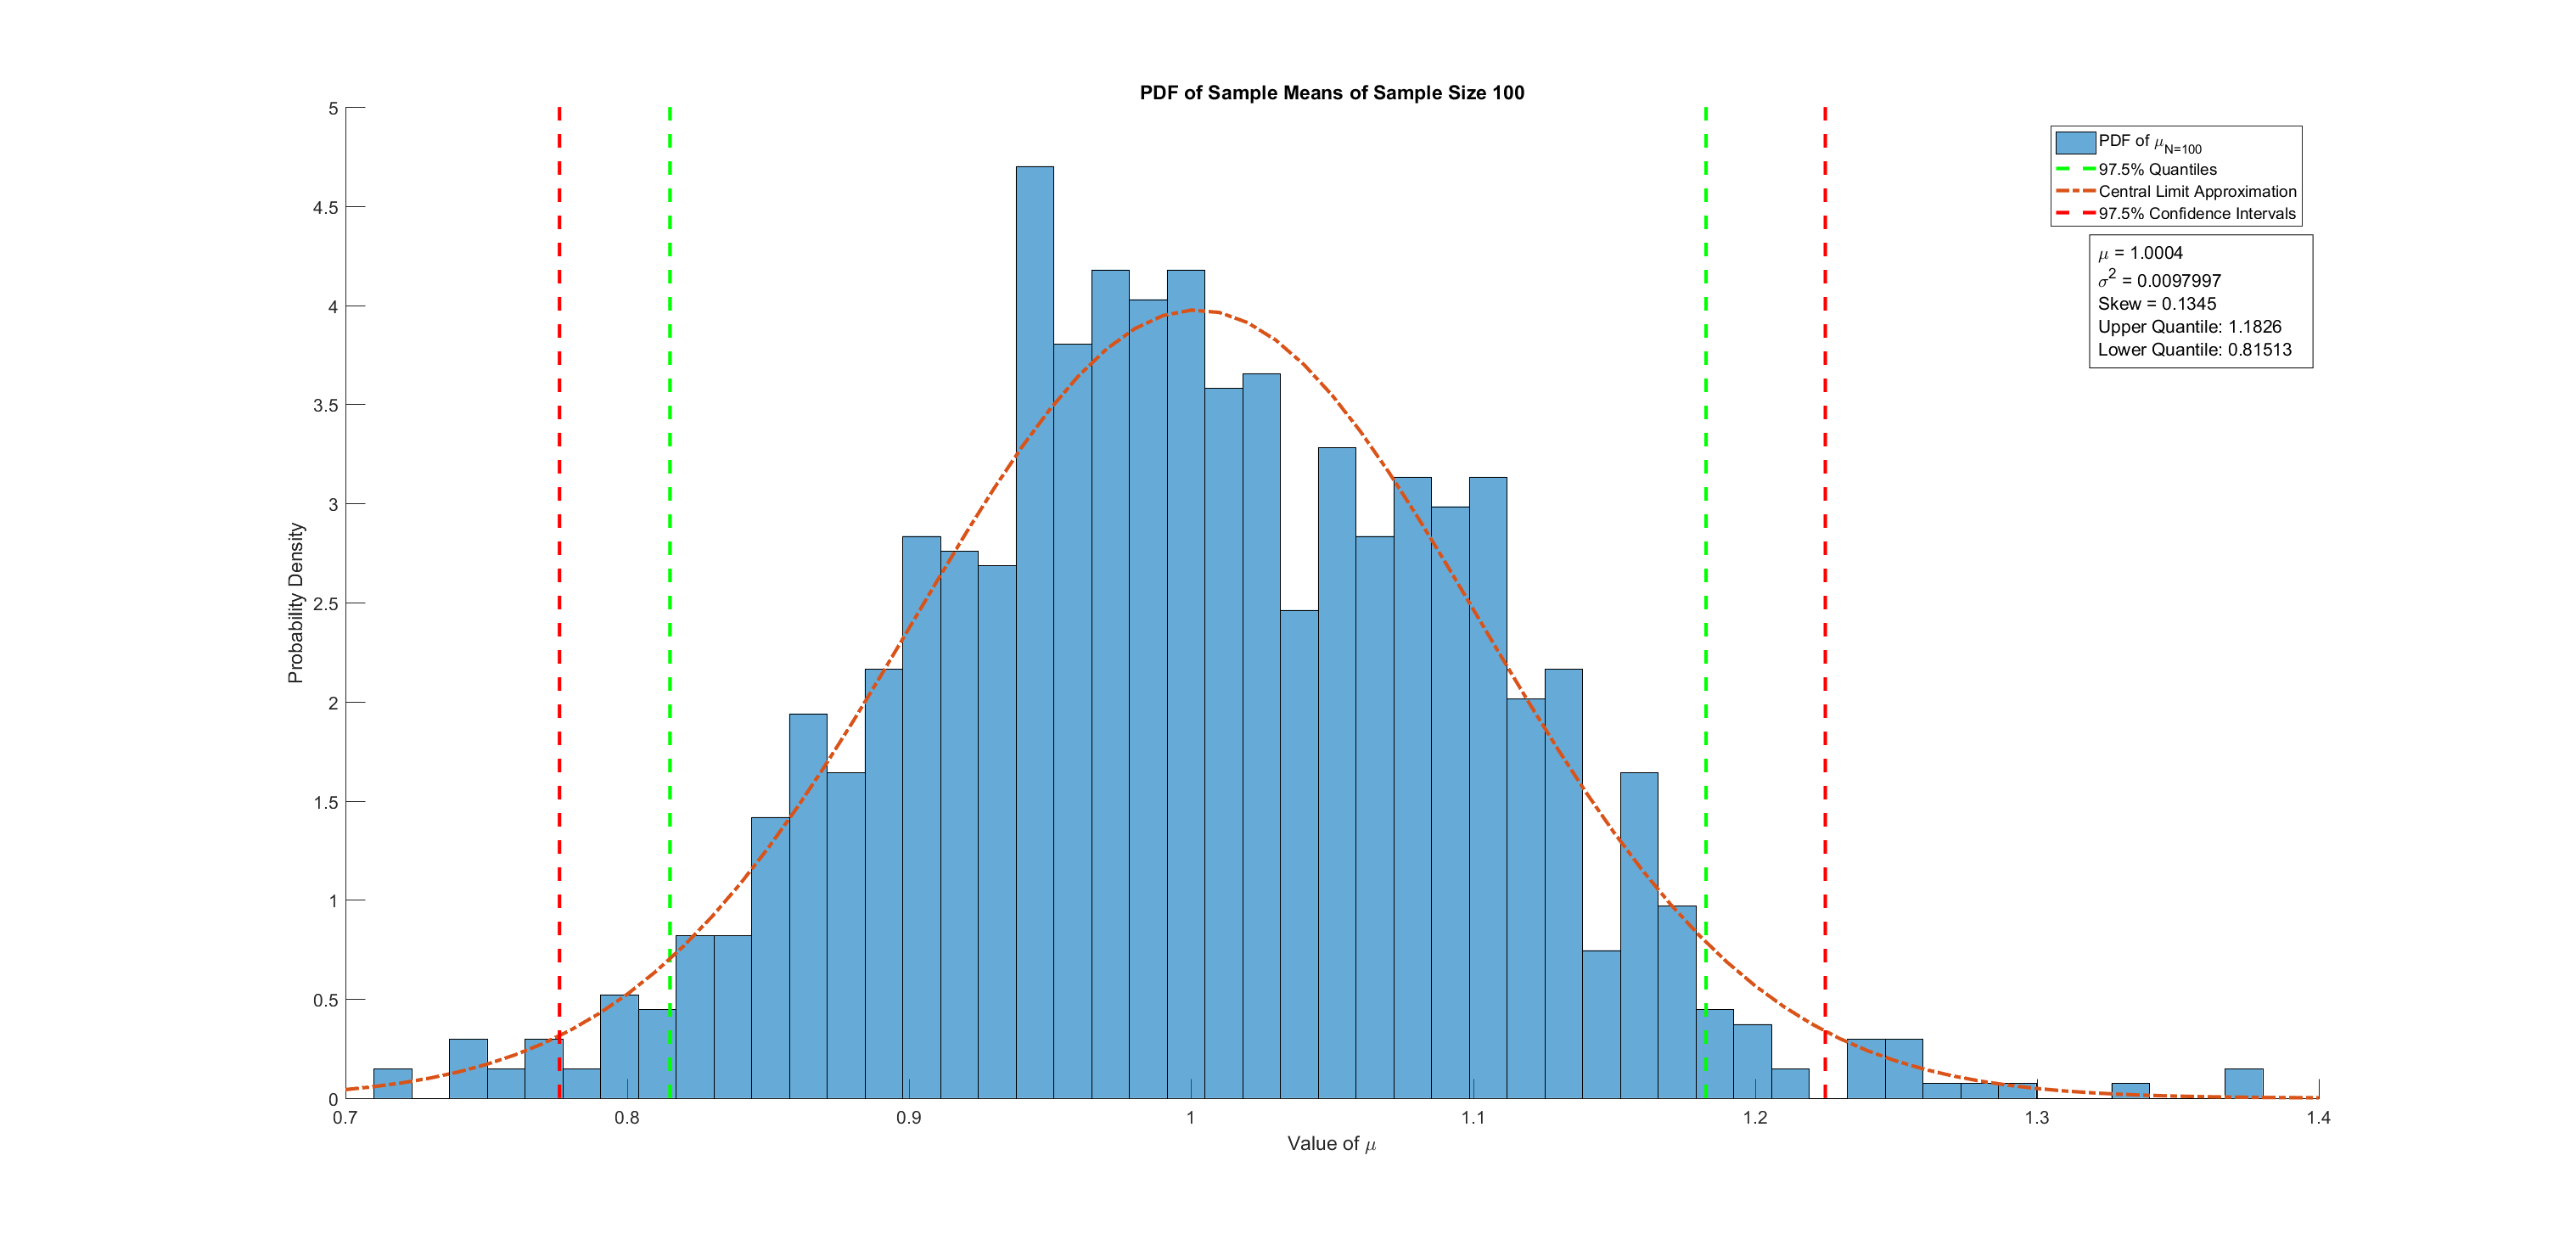
\includegraphics [width=\textwidth]{prob4_06.eps}

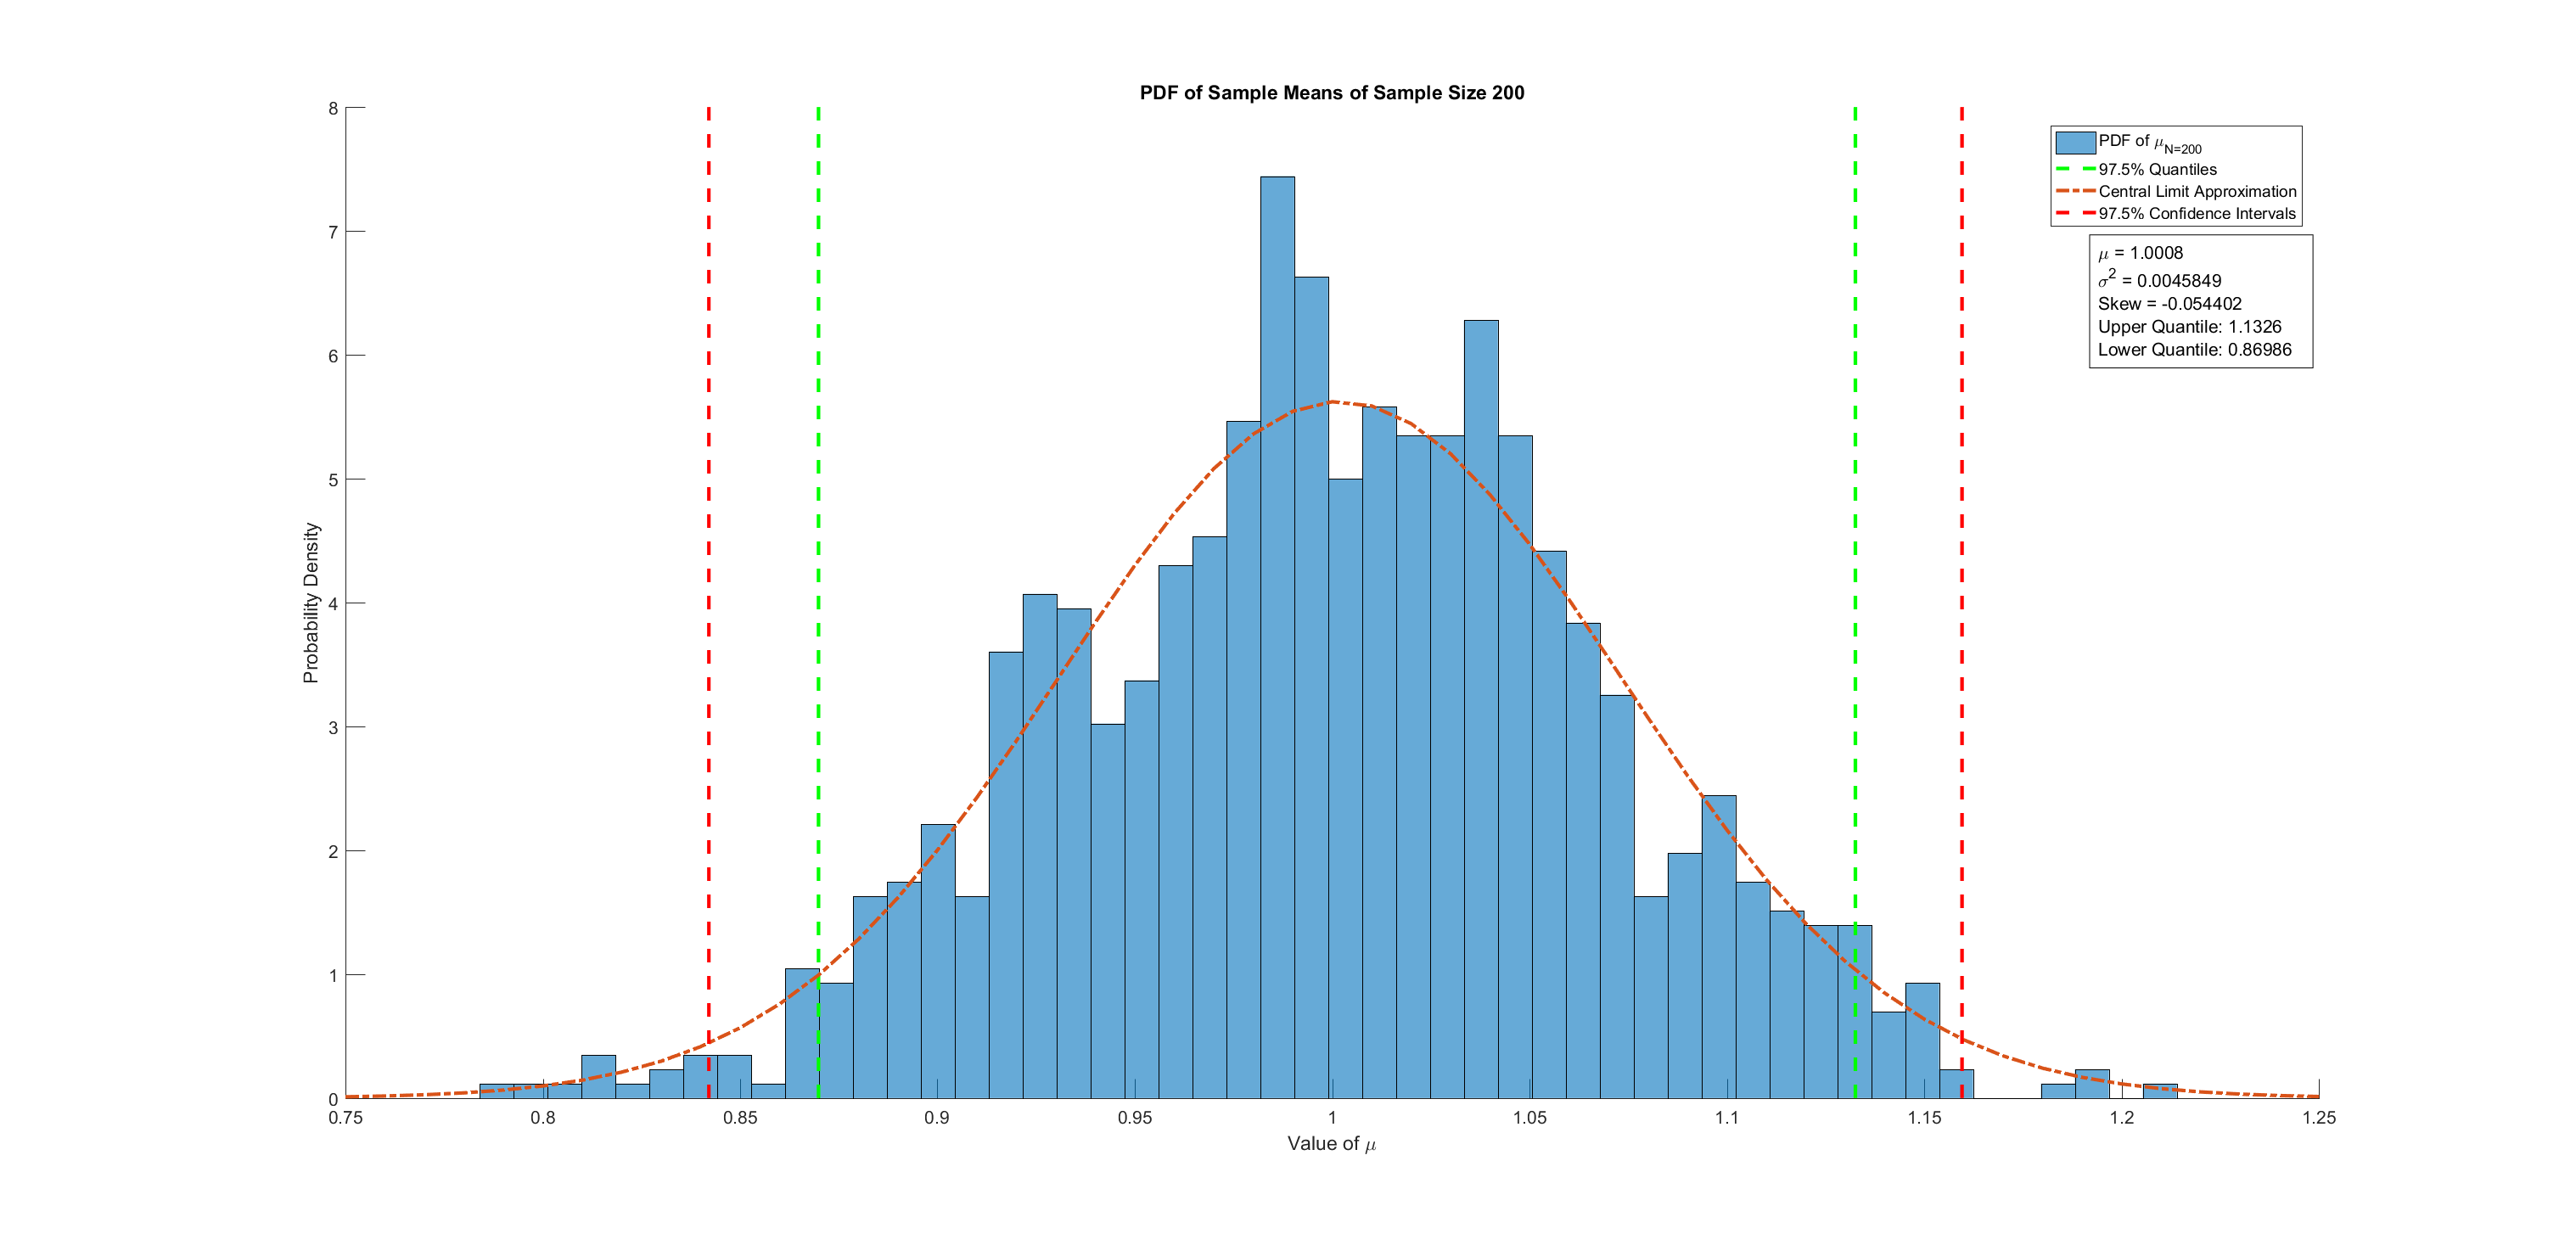
\includegraphics [width=\textwidth]{prob4_07.eps}

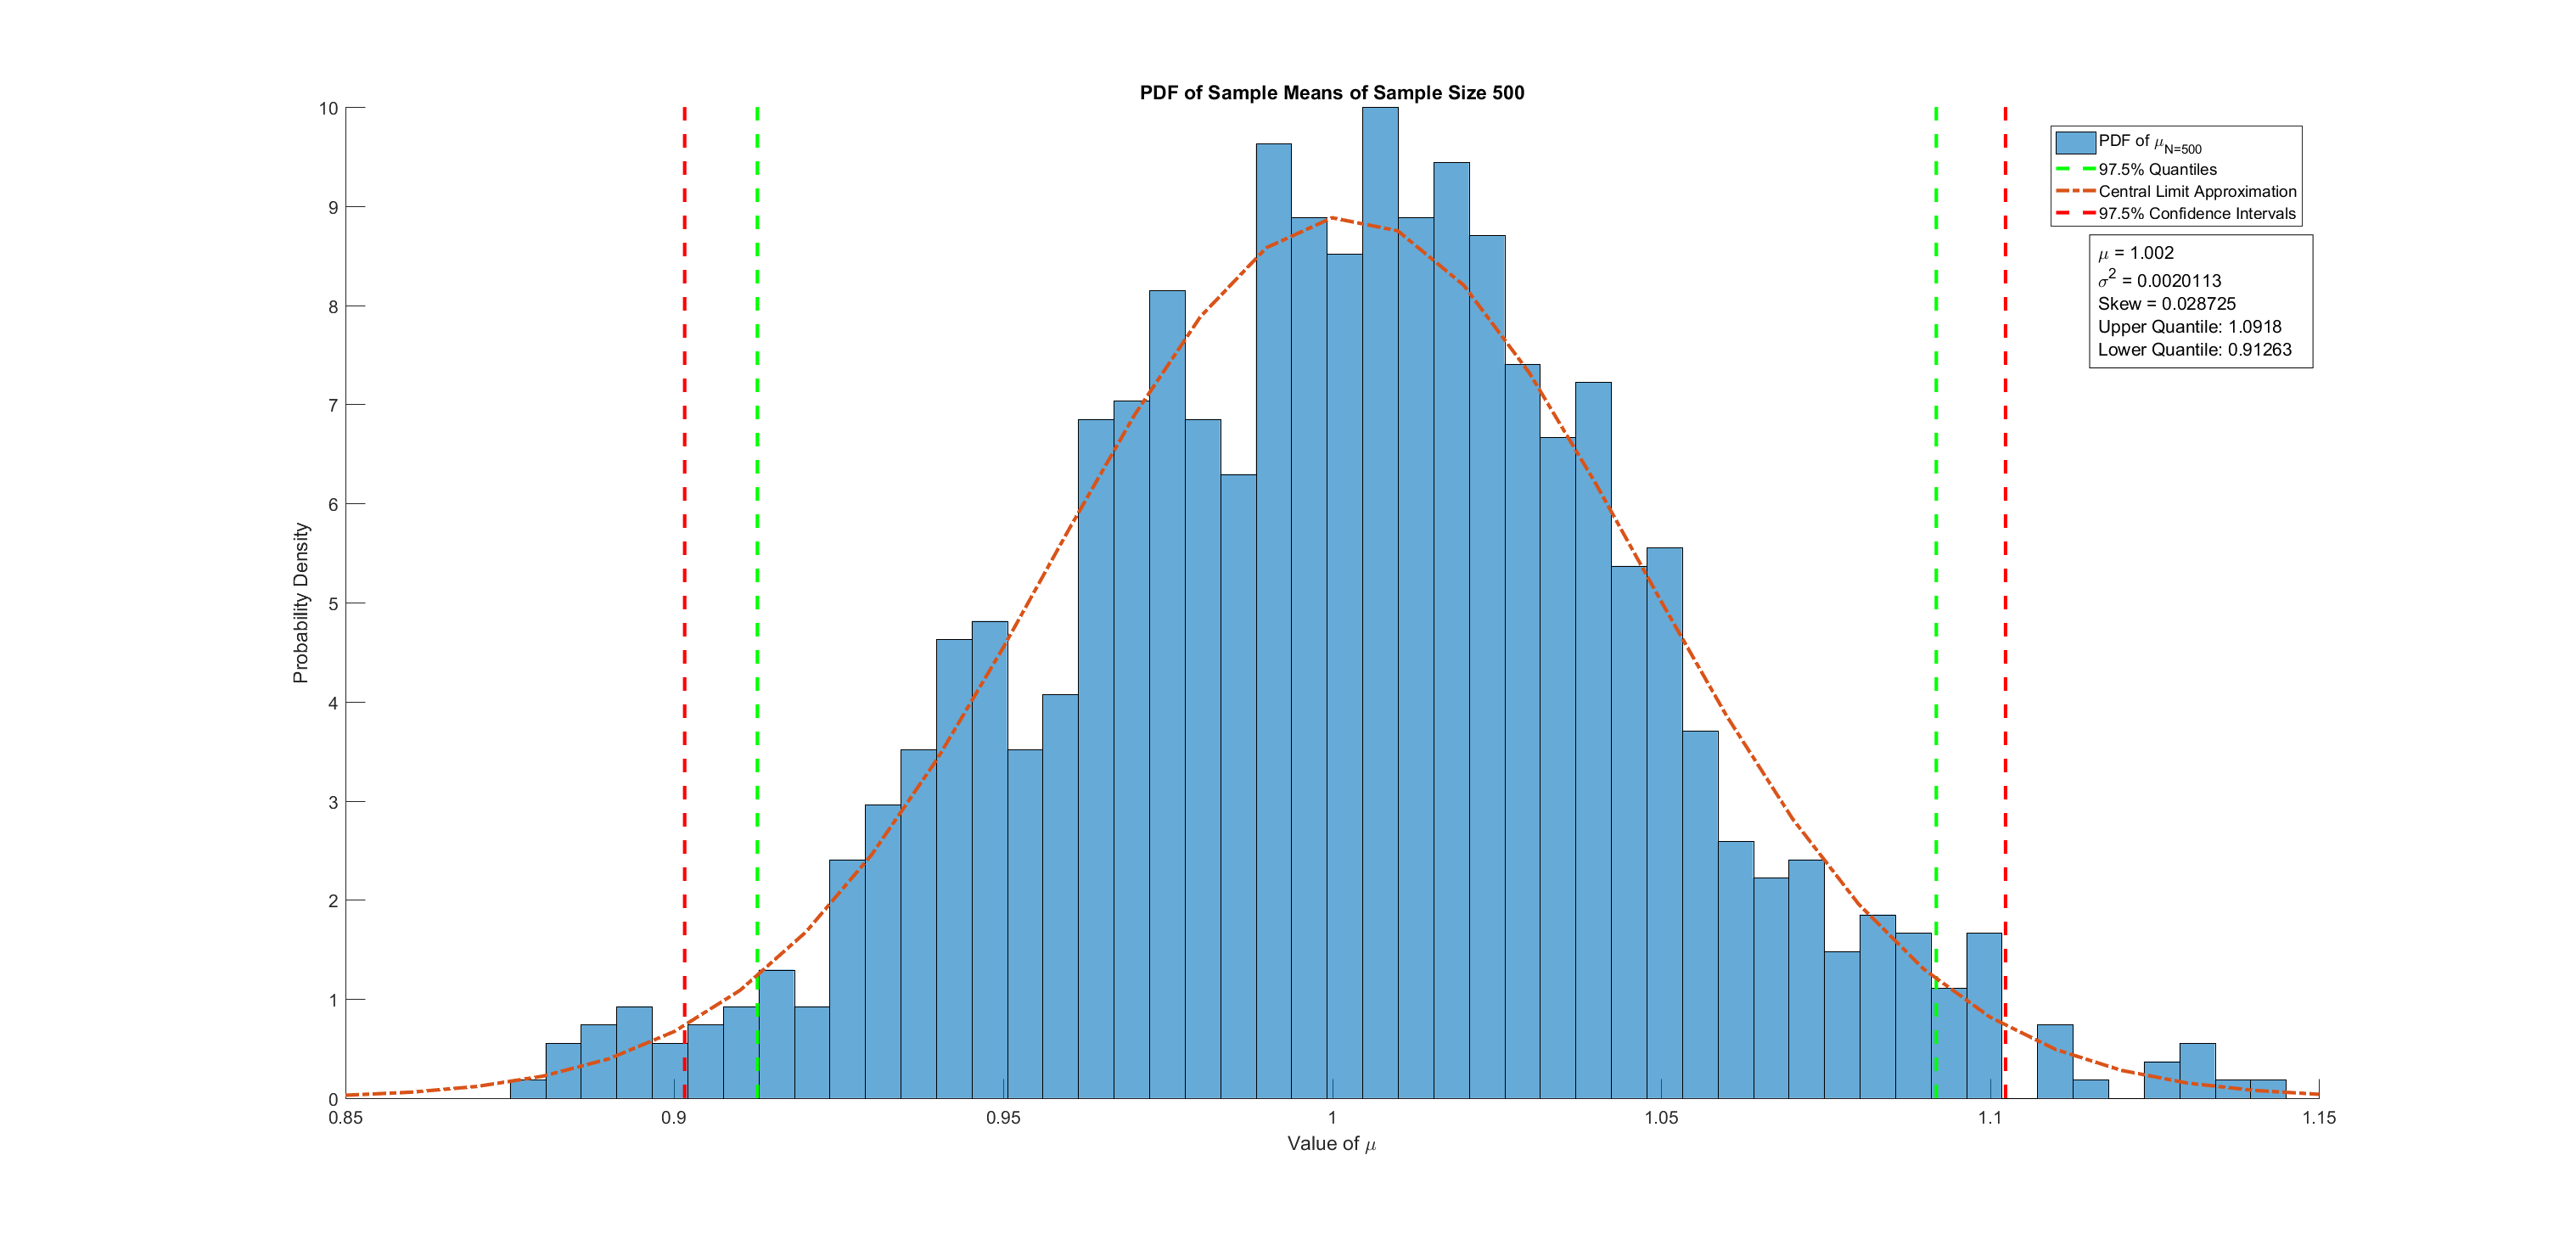
\includegraphics [width=\textwidth]{prob4_08.eps}

\end{document}
